\documentclass[12pt,b5paper]{ltjsarticle}

%\usepackage[margin=15truemm, top=5truemm, bottom=5truemm]{geometry}
%\usepackage[margin=10truemm,left=15truemm]{geometry}
\usepackage[margin=10truemm]{geometry}

\usepackage{amsmath,amssymb}
%\pagestyle{headings}
\pagestyle{empty}

%\usepackage{listings,url}

% 記号変更
%\renewcommand{\theenumi}{(\arabic{enumi})}
\renewcommand{\labelenumi}{(\arabic{enumi})}


%\usepackage{graphicx}

\usepackage{tikz} % draw graphics : TikZ ist kein Zeichenprogramm
\usetikzlibrary{arrows.meta}

%\usepackage{wrapfig}
%\usepackage{bm} % ベクトルの矢印

%\usepackage{luatexja-ruby} % ルビを振る

%% 核Ker 像Im Hom を定義
\newcommand{\Ker}{\mathop{\mathrm{Ker}}\nolimits}
\newcommand{\Img}{\mathop{\mathrm{Img}}\nolimits}
%\newcommand{\Hom}{\mathop{\mathrm{Hom}}\nolimits}

%\DeclareMathOperator{\Rot}{rot}
%\DeclareMathOperator{\Div}{div}
%\DeclareMathOperator{\Grad}{grad}
%\DeclareMathOperator{\arcsinh}{arcsinh}
%\DeclareMathOperator{\arccosh}{arccosh}
%\DeclareMathOperator{\arctanh}{arctanh}

\usepackage{url} % URLの記述

%\usepackage{listings}
%
%\lstset{
%%プログラム言語(複数の言語に対応,C,C++も可)
%  language = Python,
%%  language = Lisp,
%%  language = C,
%  %背景色と透過度
%  %backgroundcolor={\color[gray]{.90}},
%  %枠外に行った時の自動改行
%  breaklines = true,
%  %自動改行後のインデント量(デフォルトでは20[pt])
%  breakindent = 10pt,
%  %標準の書体
%%  basicstyle = \ttfamily\scriptsize,
%  basicstyle = \ttfamily,
%  %コメントの書体
%%  commentstyle = {\itshape \color[cmyk]{1,0.4,1,0}},
%  %関数名等の色の設定
%  classoffset = 0,
%  %キーワード(int, ifなど)の書体
%%  keywordstyle = {\bfseries \color[cmyk]{0,1,0,0}},
%  %表示する文字の書体
%  %stringstyle = {\ttfamily \color[rgb]{0,0,1}},
%  %枠 "t"は上に線を記載, "T"は上に二重線を記載
%  %他オプション:leftline,topline,bottomline,lines,single,shadowbox
%  frame = TBrl,
%  %frameまでの間隔(行番号とプログラムの間)
%  framesep = 5pt,
%  %行番号の位置
%  numbers = left,
%  %行番号の間隔
%  stepnumber = 1,
%  %行番号の書体
%%  numberstyle = \tiny,
%  %タブの大きさ
%  tabsize = 4,
%  %キャプションの場所("tb"ならば上下両方に記載)
%  captionpos = t
%}

%\usepackage{cancel}
%\usepackage{bussproofs}
%\usepackage{proof}

\begin{document}



\begin{center}
 \begin{tabular}{|c|c|c|c|}
  & $x < 1$ & $1\leq x < 3$ & $x\geq3$\\
  \hline
  $C_{1}$ & $50\%$ & $35\%$ & $15\%$ \\
  $C_{2}$ & $48\%$ & $16\%$ & $36\%$
 \end{tabular}
\end{center}

カテゴリ$C_{1},C_{2}$

$C_{2}$の中を$A$とそれ以外に分ける

$A$は$C_{2}$の6割である

$C_{2}$の中の$A$以外部分の分布は$C_{1}$と等しい

\begin{center}
 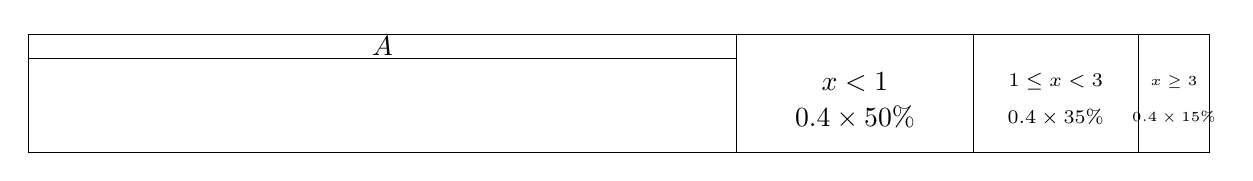
\begin{tikzpicture}[scale=0.15]
  \draw (0,0) -- (100,0) -- (100,10) -- (0,10) -- cycle;
  \draw (60,0) -- (60,10);

  \draw (0,8) -- (60,8);
  \draw (30,9) node {$A$};

  \draw (80,0) -- (80,10);
  \draw (70,6) node {$x<1$};
  \draw (70,3) node {$0.4 \times 50\%$};

  \draw (94,0) -- (94,10);
  \draw (87,6) node {\scriptsize$1\leq x<3$};
  \draw (87,3) node {\scriptsize$0.4 \times 35\%$};

  \draw (97,6) node {\tiny$x\geq3$};
  \draw (97,3) node {\tiny$0.4 \times 15\%$};

 \end{tikzpicture}
\end{center}

$C_{2}$には$x<1$が$48\%$あるが、
$A$に属しない部分には$0.4\times 0.5 = 20\%$あるため、
$A$の中の$x<1$は$28\%$となる

同様に
$A$の中の$1\leq x<3$は$0.16-0.4\times 0.35 = 2\%$となる

$A$の中の$x\geq3$は$0.36-0.4\times 0.15 = 30\%$となる

$C_{2}$のうち$A$の割合が6割なので、
次のような割合になっている。
\begin{center}
 [$x<1$] $28\%$
 ,\qquad
 [$1\leq x<3$] $2\%$
 ,\qquad
 [$x\geq 3$] $30\%$
\end{center}

これを$A$を$100\%$として計算し直す
\begin{center}
 [$x<1$] $28\% \div 0.6 = \frac{28}{60}$
 ,\qquad
 [$1\leq x<3$] $2\% \div 0.6 = \frac{2}{60}$
 ,\qquad
 [$x\geq 3$] $30\% \div 0.6 = \frac{30}{60}$
\end{center}

%集団$A$には$x<3$と$x\geq 3$が次のように存在する。
%\begin{center}
%[$x < 3$] $\frac{30}{60}$
% \qquad
% [$x\geq 3$] $\frac{30}{60}$
%\end{center}


この集団$A$から$16$個を取り出し、
$6$個が$x<3$である確率は計算で求められる。
特に、6個以下である確率は次の式で求められる。
\begin{equation}
 \sum_{i=0}^{6} {}_{16}C_{i} \left(\frac{1}{2}\right)^{i} \left(\frac{1}{2}\right)^{16-i}
\end{equation}

つまり、
二項分布$B\left( 16,\frac{1}{2} \right)$にしがたう。
(上記計算結果は$0.2272491\dots$となる。)

二項分布$B(n,p)$は
取り出した個数$n$が
十分に大きいと
正規分布$N(np,np(1-p))$で近似できる。

今の場合、$n=16,p=1/2$であるから
$N(8,4)$で近似できるとする。


そこで標準化$Z=(X-\mu)/\sigma$を行う。
\begin{equation}
 Z=\frac{6-8}{\sqrt{4}} = -1
\end{equation}

この値を正規分布表から探せば
値$0.1587$が得られる。









\hrulefill



\end{document}
